\chapter{Określanie lokalizacji}
\label{cha:lokalizacja}
\section{Lokalizacja użytkownika}
Lokalizacja użytkownika w systemie określa się na podstawie odległości od punktów, których współrzędne w przestrzeni trójwymiarowej są znane. Są to głównie routery i Beacony, jednak może się zdarzyć, że takim punktem staje się również inny użytkownik. Współrzędne użytkownika można obliczyć, podając siły sygnałów odebranych przez otaczające go urządzenia i obliczając na ich podstawie dystans.
\section{Trilateracja}
Najbardziej znanym sposobem obliczenia lokalizacji użytkownika na podstawie dystansu do znanych punktów jest trilateracja. Metoda ta polega na przedstawienie dystansu dzielącego punkt od nadajników jako okręgi (lub jako sfery w przypadku, gdy określamy lokalizację w trzech wymiarach). Następnie, należy wyznaczyć współrzędne punktu przecięcia okręgów. Wyznaczone współrzędne są lokalizacją punktu, dla którego dokonywaliśmy obliczenia.
\begin{figure}[H]			
	\centering
	\caption{Wizualizacja modelu trilateracji}
	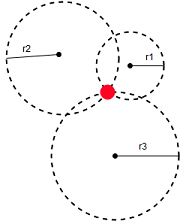
\includegraphics{trilateracja}
\end{figure}
Współrzędną punktu można obliczyć na podstawie wzoru:
\begin{equation}
\left\{
\begin{array}{l}
(x_p-x_1)^2 + (y_p - y_1)^2 = r_1^2\\
(x_p-x_2)^2 + (y_p - y_2)^2 = r_2^2\\
(x_p-x_3)^2 + (y_p - y_3)^2 = r_3^2
\end{array}
\right.
\end{equation}
gdzie:
\begin{itemize}
	\item $x_p$, $y_p$ to współrzędne obliczanego punktu
	\item $x_1$, $y_1$, $x_2$, $y_2$, $x_3$, $y_3$ to współrzędne znanych punktów
	\item $r_1$, $r_2$, $r_3$ to odległości między punktem obliczanym, a punktami o znanych współrzędnych
\end{itemize}
Ta metoda lokalizowania użytkownika w przestrzeni ma jedną, bardzo ważną wadę, która wyklucza jej wykorzystanie w stworzonym systemie - nie potrafi się dostosować do błędów pomiarów, których w przypadku określania lokalizacji przy użyciu sygnałów radiowych, jest dużo. Aby obliczane lokalizację użytkowników w sposób zbliżony odwzorowywały rzeczywiste położenie, algorytm obliczający musiał być bardziej odporny na błędy pomiarowe.
\section{Lokalizacja jako funkcja probabilistyczna Gaussa}
\subsection{Funkcja probabilistyczna Gaussa}
Funkcja probabilistyczna Gaussa jest to krzywa w kształcie dzwonu, symetryczna względem średniej $\mu$ oraz uzyskująca wartość maksymalną w punkcie $\frac{1}{\sqrt{2\pi}\sigma}$.
Określa się ją za pomocą wzoru:
\begin{equation}
F(x) = \frac{1}{\sigma\sqrt{2\pi}}e^{\left(\frac{-(x-\mu)^2}{2\sigma^2}\right)}
\end{equation}
Zmienna $\mu$ będąca średnią, oraz $\sigma$ będąca odchyleniem standardowym, w pełni opisują tą funkcję.
\begin{figure}[H]			
	\centering
	\caption{Wykres funkcji Gaussa dla różnych wartości parametrów}
	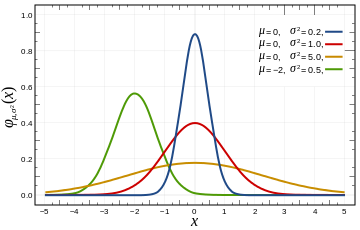
\includegraphics{funkcja_Gaussa}
\end{figure}
Funkcja Gaussa jest szeroko wykorzystywana statystyce. W elektronice, funckcja Gaussa wykorzystywana jest podczas charakteryzowania pomiarów sensorów czy siły sygnałów radiowych.
\subsection{Model routerów jako funckcja Gaussa}
Z racji tego, iż mierzony sygnał, odbierany przez odbiornik, ulega znieksztalceniom i odbiciom, określenie dystansu między transmiterem, a odbiorcą w sposób liniowy jest niezgodne z fizycznymi zachowaniami sygnału. Z racji tego, iż siła sygnału oraz straty wynikące ze zniekształceń i odbić, określone są w jednostce dB, najlepszym przybliżeniem zmian siły sygnału może być funkcja Gaussa.\\
Jeżeli określimy lokalizację obiornika względem transmitera jako funkcję prawdopodobieństwa Gaussa, to:
\begin{equation}
F(x) = \frac{1}{\sigma\sqrt{2\pi}}e^{\left(\frac{-(x-d)^2}{2\sigma^2}\right)}
\end{equation}
to wartość funkcji określa, jakie jest prawdopodobieństwo, że odbiornik znajduje się w odległości $x$ od transmitera. Największe pradopodobieństwo przypisywane jest dystansowi, który obliczyliśmy z siły sygnału, dlatego to właśnie ta wartość podstawiana jest pod zmienną $d$.\\
Jeżeli opisałoby się transmiter jako funkcję prawdopobieństwa Gaussa wyznaczonej na podstawie odebranej siły sygnału, zwizualizowany model trasmitera w przestrzeni dwuwymiarowej przypominałby pierścień, którego siła malałaby wraz z oddalaniem się od obliczonej odległości.
\begin{figure}[H]			
	\centering
	\caption{Wizaulizacja modelu routera opisanego funkcją Gaussa}
	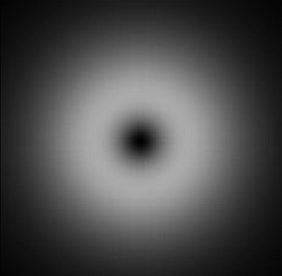
\includegraphics{router_Gaussa_wizualizacja}
\end{figure}
\subsection{Lokalizacja użytkownika opisana funkcją Gaussa}
Wyżej opisane podejście, poza realistyczniejszym oddaniem natury rozchodzenia się sygnału w środowisku, ma również dodatkową zaletę - w łatwy sposób można wyliczyć prawdopodobieństwo określające położenie odbiornika w sytuacji, gdy w modelu znajduje się więcej transmiterów.\\
Jednym ze sposobów określania położenia użytkownika jest zsumowanie prawdopodobieństw obliczony z funkcji Gaussa każdego z transmiterów dla każdego punktu w przestrzeni. Prawdopobieństwo dla puntu $(X,Y)$ może być określone na podstawie wzoru:
\begin{equation}
F(X,Y) = \sum_{r=1}^{r=R} \frac{1}{\sigma\sqrt{2\pi}}e^{\left(\frac{-(D(X,Y,r)-d_r)^2}{2\sigma^2}\right)}
\end{equation}
w którym kolejne symbol oznaczają:
\begin{itemize}
	\item $R$ - zbiór transmiterów. Z racji tego, iż funkcja Gaussa przyjmuje wartości dodatnie dla całego zakresu $(-\infty,\infty)$, wartość prawdopodobieństwa jest liczona dla każdego transmitera, niezależnie od tego, jak daleko znajduje się on od punktu $(X,Y)$
	\item $D(X,Y,r)$ - euklidesowa odległość punktu $(X,Y)$ od transmitera
	\item $d_r$ - odległość obliczona na podstawie siły sygnału transmitera $r$
\end{itemize}
Po ustaleniu wartości dla wszystkich punktów $(X,Y)$ w przestrzeni, jako lokalizacja odbiornika przyjęty zostaje taki punkt $(X_o,Y_o)$, którego suma prawdopodobieństwa jest największa.
\begin{figure}[H]			
	\centering
	\caption{Model lokalizacji odbiornika wykonany w programie MatLab. Punkt o największym prawdopodobieństwie oznaczony jest za pomocą czarnej strzałki.}
	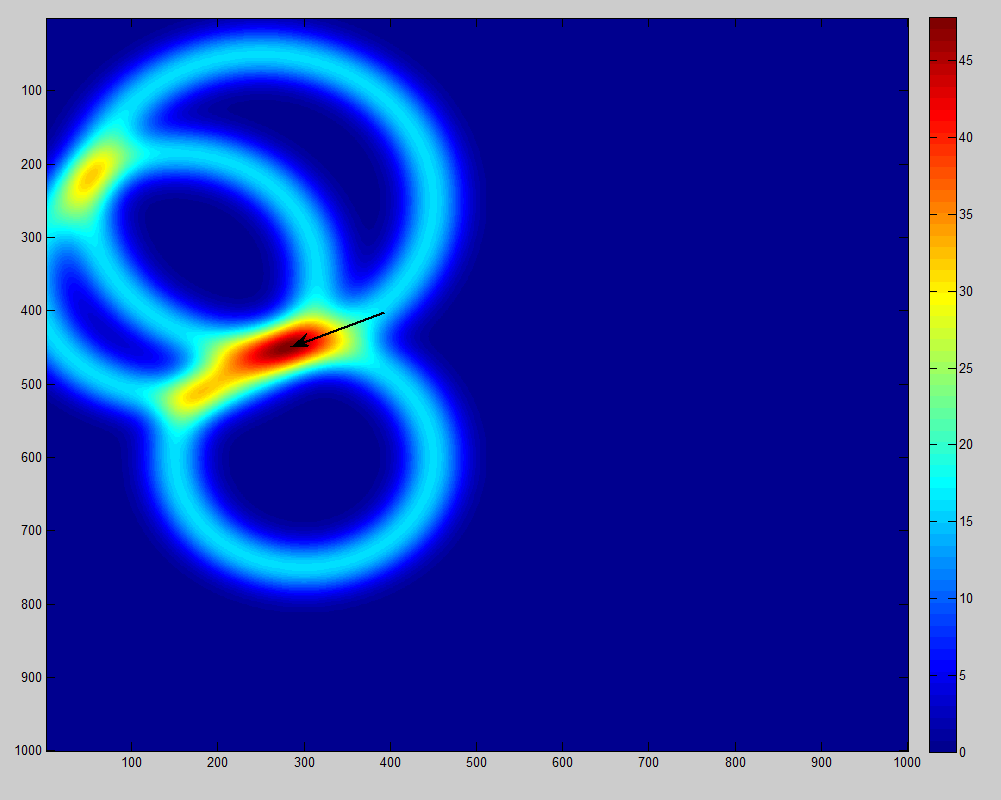
\includegraphics[width=0.75\textwidth]{guasianRouter}
\end{figure}
Zaprezentowany sposób wyznaczania lokalizacji dotyczył lokalizacji w przestrzeni dwuwymiarowej. Przejście na obliczenia w przestrzeni trójwymiarowej nie stanowią problemu - jedynymi zmianami, jakie należy wykonać są:
\begin{itemize}
	\item dokonywanie obliczeń dla punktów $(X,Y,Z)$
	\item zmiana sposobu obliczania odległości euklidesowej między odbiornikiem, a transmiterem - należy wyznaczać odległość w przestrzeni trójwymiarowej.
\end{itemize}
